\problemname{Mountain Hike}

\begin{figure}[ht!]
  \centering
  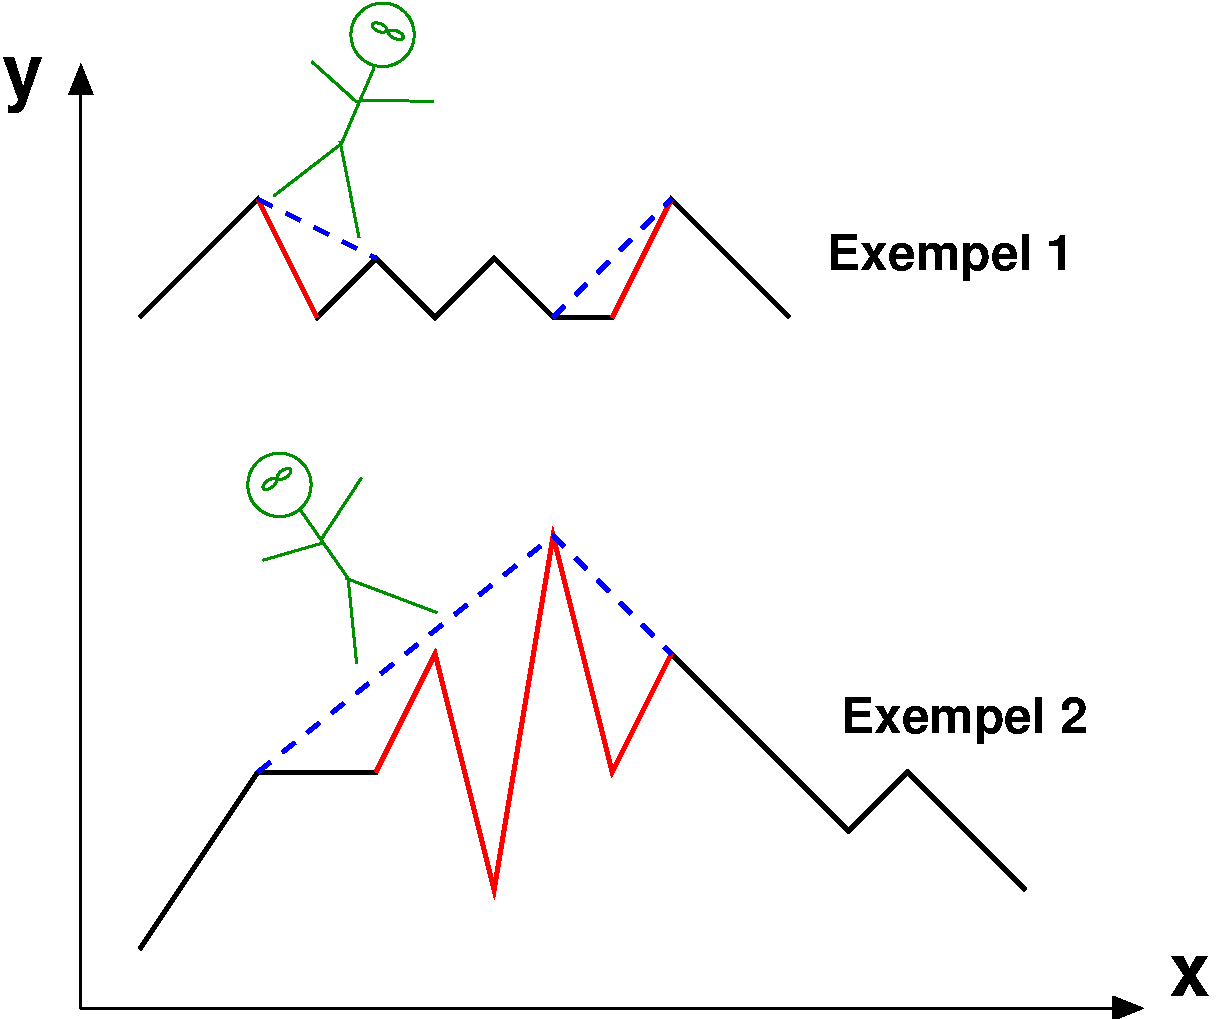
\includegraphics[width=0.4\textwidth]{berg.pdf}
  \caption{The shape of the mountain in samples $1$ and $2$. The red segments are too steep to walk on. The dashed blue lines are bridges that the hikers build.}
\end{figure}

A mountain range consists of $n$ points, ($x_1$, $y_1$) to ($x_n$, $y_n$), where $x_1 < x_2 < \dots < x_n$. Between point $i$ and point $i+1$ there is a line segment.

Some hikers want to cross the entire mountain range, that is, walk from point $1$ to point $n$. However, they cannot walk on a line segment if its slope is strictly greater than $d$. Here we define the slope of the line through ($x_i$, $y_i$) and ($x_j$, $y_j$) as

$$
\frac{|y_i - y_j|}{|x_i - x_j|}
$$
where $|x|$ denotes the absolute value of $x$.

To make the hike possible, they can build bridges in the mountain range. A bridge is also represented as a line segment, and is always built between two points $i$ and $j$. A bridge may of course not have a slope greater than $d$, and furthermore it is not possible to build a bridge that passes through the mountain at any place.

Determine the minimum total length of the bridges that need to be built in order to make the hike possible.

\section*{Input}
The first line contains the integer $n$ and the floating-point number $d$ ($2 \leq n \leq 1000$, $0 < d \le 10^5$).
$d$ is given with at most three decimals of precision.

The following $n$ lines each contain two integers $0 \leq x_i, y_i \le 10^6$, the coordinates of point $i$, also separated by a space. It is guaranteed that $x_i < x_{i+1}$.

\section*{Output}
Print a floating-point number: the minimum total length of bridges needed to make the hike possible.
If it is impossible to complete the hike no matter how the bridges are built, print $-1$ instead.

Your answer will be accepted if the absolute error is less than $10^{-3}$.
It is guaranteed that the result for a test case is not affected by a \emph{small} change of the number $d$ (this is to avoid precision errors when comparing floating-point numbers).

\section*{Scoring}
Your solution will be tested on a set of test groups.
To earn points for a group, you must pass all test cases in that group.

\noindent
\begin{tabular}{| l | l | p{12cm} |}
  \hline
  \textbf{Group} & \textbf{Points} & \textbf{Constraints} \\ \hline
  $1$    & $40$        & $n \leq 100$ \\ \hline
  $2$    & $60$        & No additional constraints.  \\ \hline
\end{tabular}
